Overview of this part.

\chapter{Memory Object Models, explained}\label{chap:mem-model-explained}

Explain the connection to Core \textemdash{} not that strong, thanks to the memory
interface and the invariants of the VIP heaps, separation logic heaps, and
memory actions.

Factorising the formalisation pays off here.

\chapter{Pointers: more than you wanted to know}

Explain pointers in excrutiating detail, and why we need provenance for
optimisations.

Why do we care about provenance, why are pointers not just addresses

Common-subexpression elimination, copy-propogation, etc.

\section{Explaining PNVI-ae-udi and VIP}

Why you need provenance.

\section{Design Space}

Alternatives

\begin{figure}[h]
    \centering
    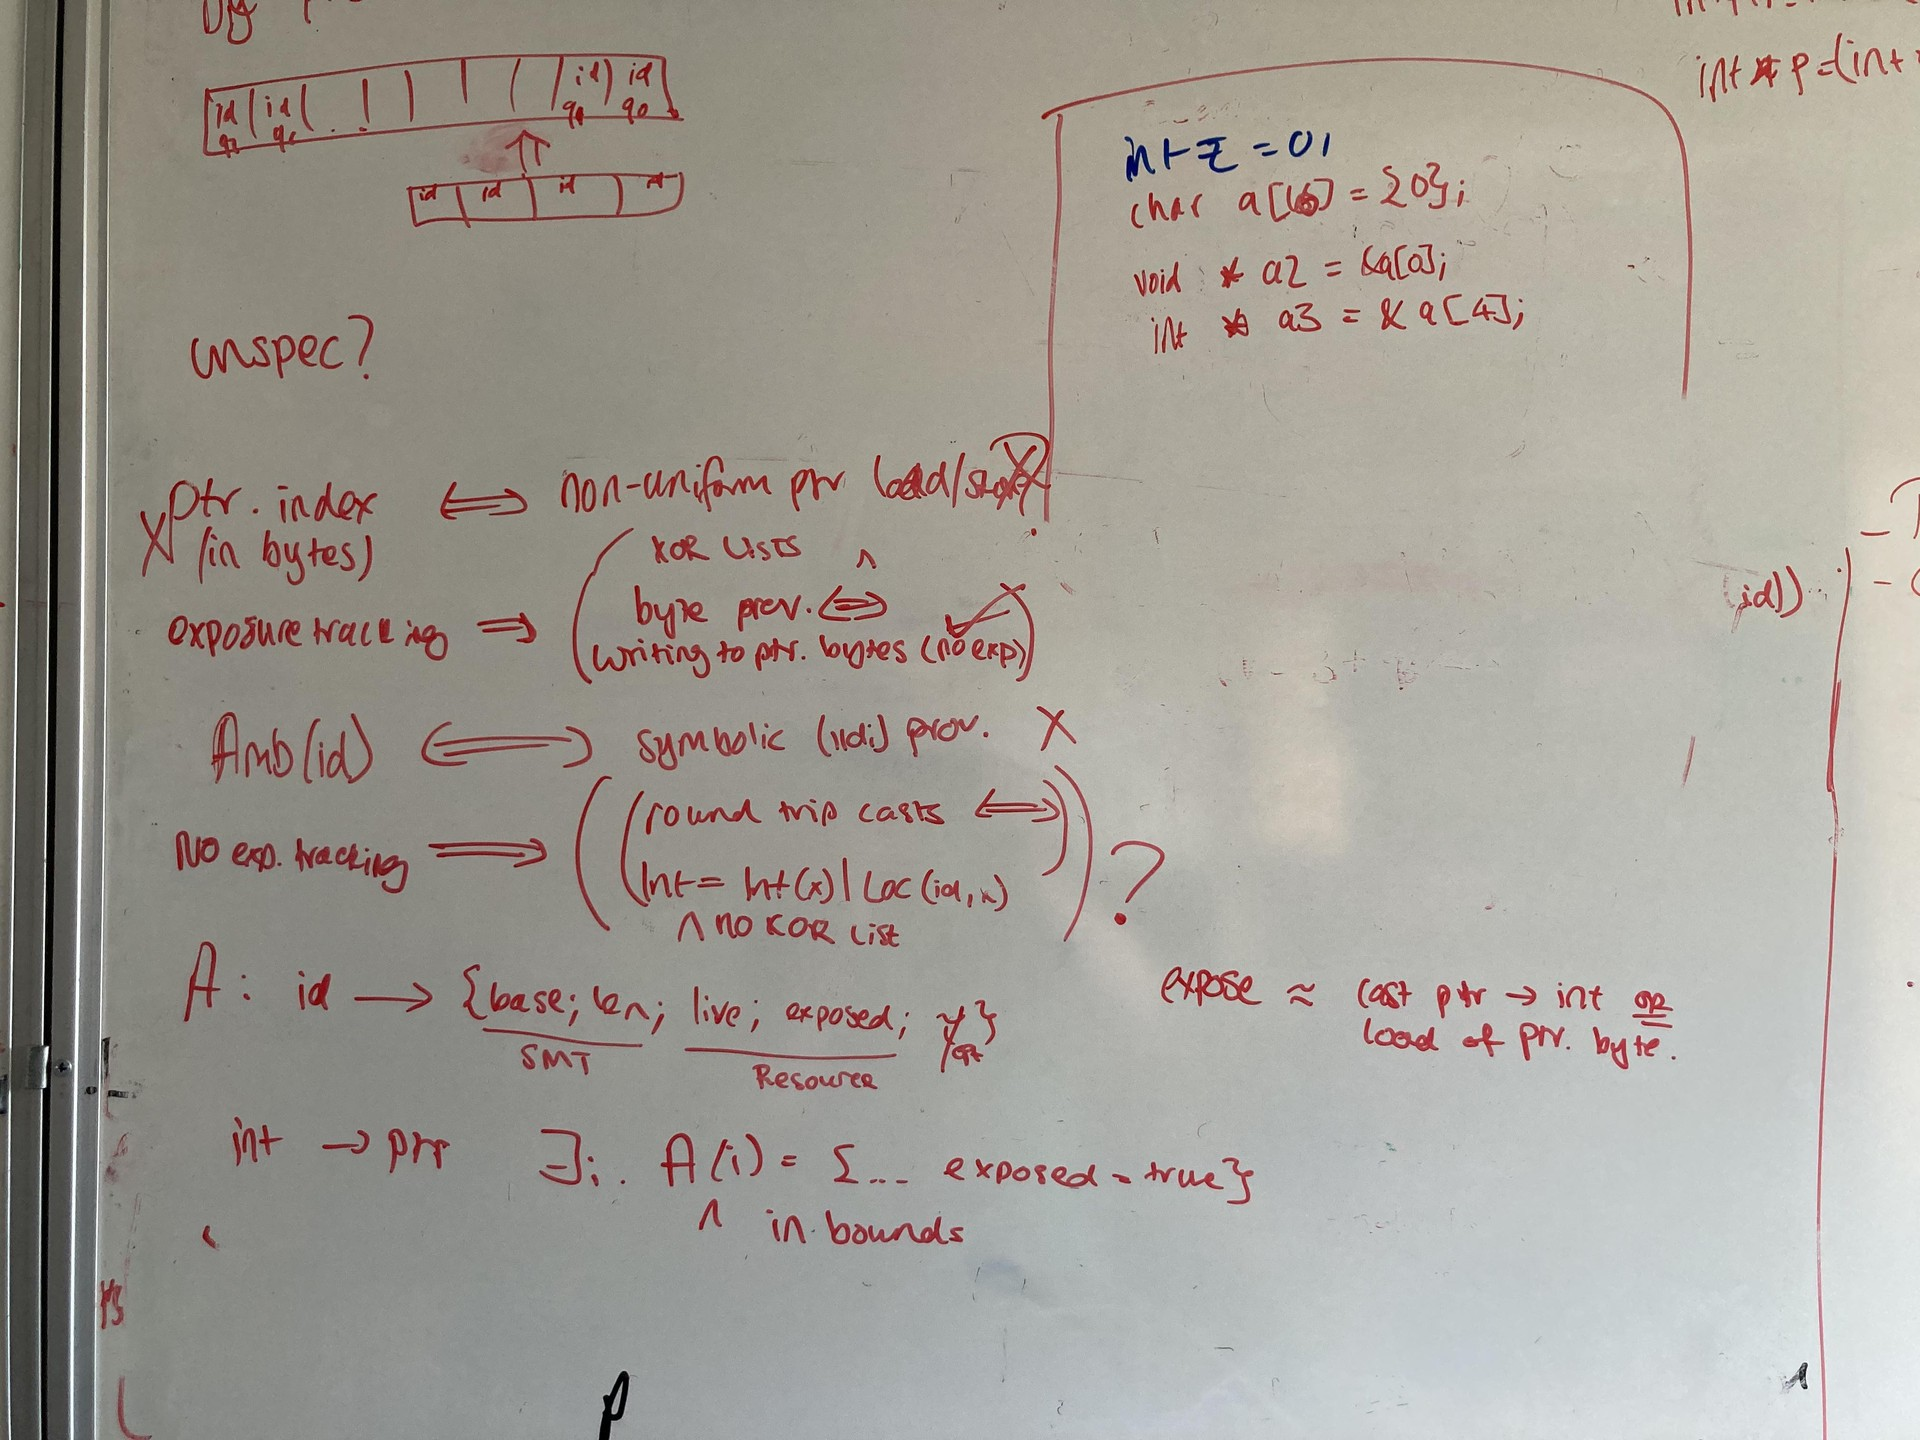
\includegraphics[width=\textwidth]{../misc/type-system-options.jpg}
\end{figure}

\section{CN-VIP}\label{sec:cn-vip}

\section{Soundness}\label{sec:cn-vip-soundness}

\section{Implementation}

Performance graph

\begin{figure}[h]
    \centering
    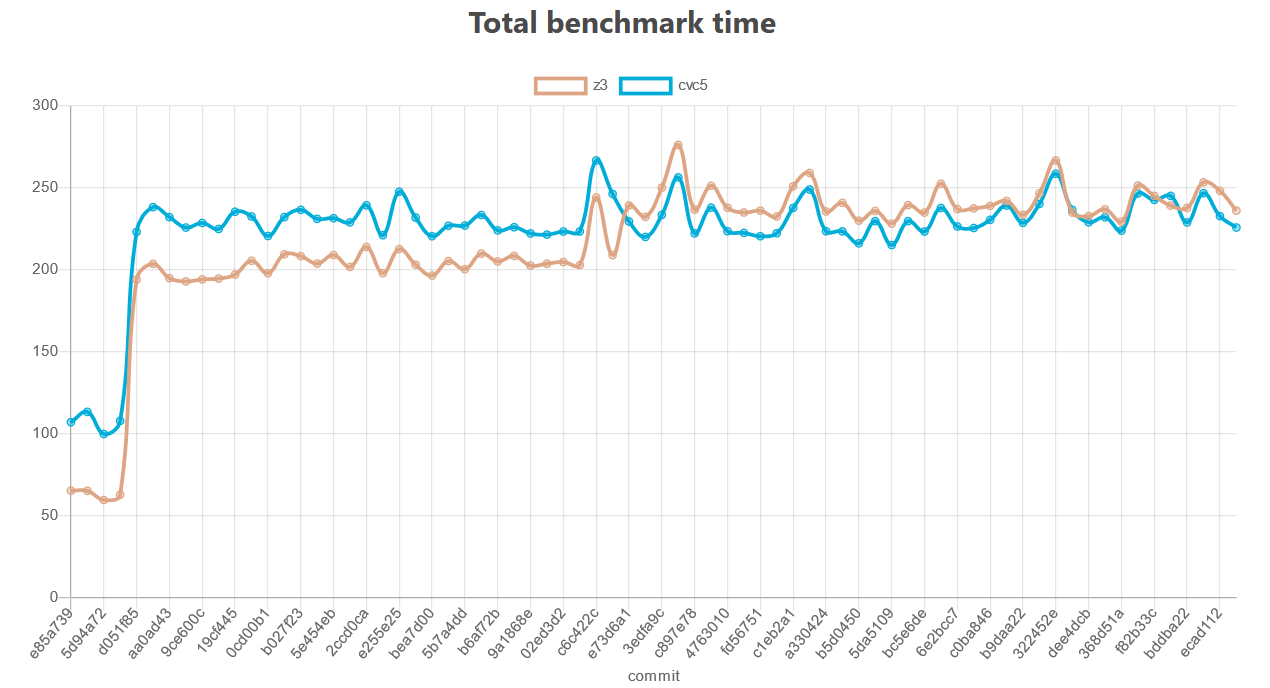
\includegraphics[width=\textwidth]{../misc/vip-performance-hit.png}
\end{figure}

\url{https://rems-project.githb.io/cerberus/dev/bench/}

\section{Translating resource lemmas}\label{sec:trans-res-lemmas}

Is there a reason, in the discussion about Cassia's PhD, we thought all of
Cerberus needed to be shoved into Iris instead of just a trace of memory model
(and eventually, concurrency) events?

irisification (cf
\url{https://people.mpi-sws.org/~dreyer/papers/iris-ground-up/paper.pdf}).  Either
just the resource algebra or (as DM suggests) also the abstract language of
memory model interface events: which one let one formalise the primitive
resource-context manipulations that CN does (conceivably extractably).

I think a sufficient halfway point would be the language of traces memory
events i.e.\ memory model as the dynamics. Resource algebra would be CN's view
of resources. Resource lemmas are then just statements saying that one resource
represents exactly the same heap as another resource (skips). Changes to the
resource algebra because of memory events (which we could introduce unsoundness
in CN) would be proved sound in Iris.

As a bonus, we could even formalise and prove sounds the inference procedures
CN uses (and with some engineering to handle SMT, even extract from Rocq).

The inference I'm talking about is resource context manipulations: checking if
we can pack or unpack predicates, if an owned is in the context, shifting
indices in and out of iterated predicates, exploding and imploding structs.
These operations don't require core structure.

Even if full extraction of the inference algo is not feasible (it would
involves standard data structures + SMT FFI), having a defined set of resource
manipulation primitives proved sound and extracting those (just standard data
structure manipulations), or even just proving the primitives sound and using a
similar interface would increase confidence.

If ones reads the above in reverse, it even provides a gradual migration path
which doesn't commit us to any next step and allows us to see how far
extraction can take us.

If the inference algs or the primitives are formalised, then we can iterate on
cleverer  inference schemes with a strong safety net

I think it will become more valuable as soon as we start having fancier things
like higher-order resources, locks, fractional permissions. At that point,
checking the steps/moves that any inference algorithm could take would get
closer to essential.

Even if an arbitrary inference algorithm is not stable, the steps available and
the shape of the resources should be more so, and that is worth at least
creating a clean abstraction for (and then pen-paper soundness, and then
mechanised soundness).

Noted and agreed that anything mechanised takes longer than one wants/expects
and that extraction is a pain. But this gives us a concrete use-case,
reasonable sequence of experiments and a clear idea of the benefits and costs.

